\documentclass[a4paper,12pt]{article}

% Packages
\usepackage[utf8]{inputenc}
\usepackage[english]{babel}
\usepackage{amsmath}
\usepackage{amssymb}
\usepackage{graphicx}
\usepackage{geometry}
\usepackage{float}
\usepackage{caption}
\usepackage{booktabs}
\usepackage{pdfpages}
\usepackage{hyperref}

% Page layout
\geometry{margin=1in}

% Title and Author
\title{Rakéták, rakéta hajtóművek\\ 2. házifeladat javítás}
\author{Ábrók László Patrik\\ JPWF8N}
\date{2025.06.10.} % Date of submission
%\date{\today}

\begin{document}

% Title Page
\maketitle
%\tableofcontents
\newpage

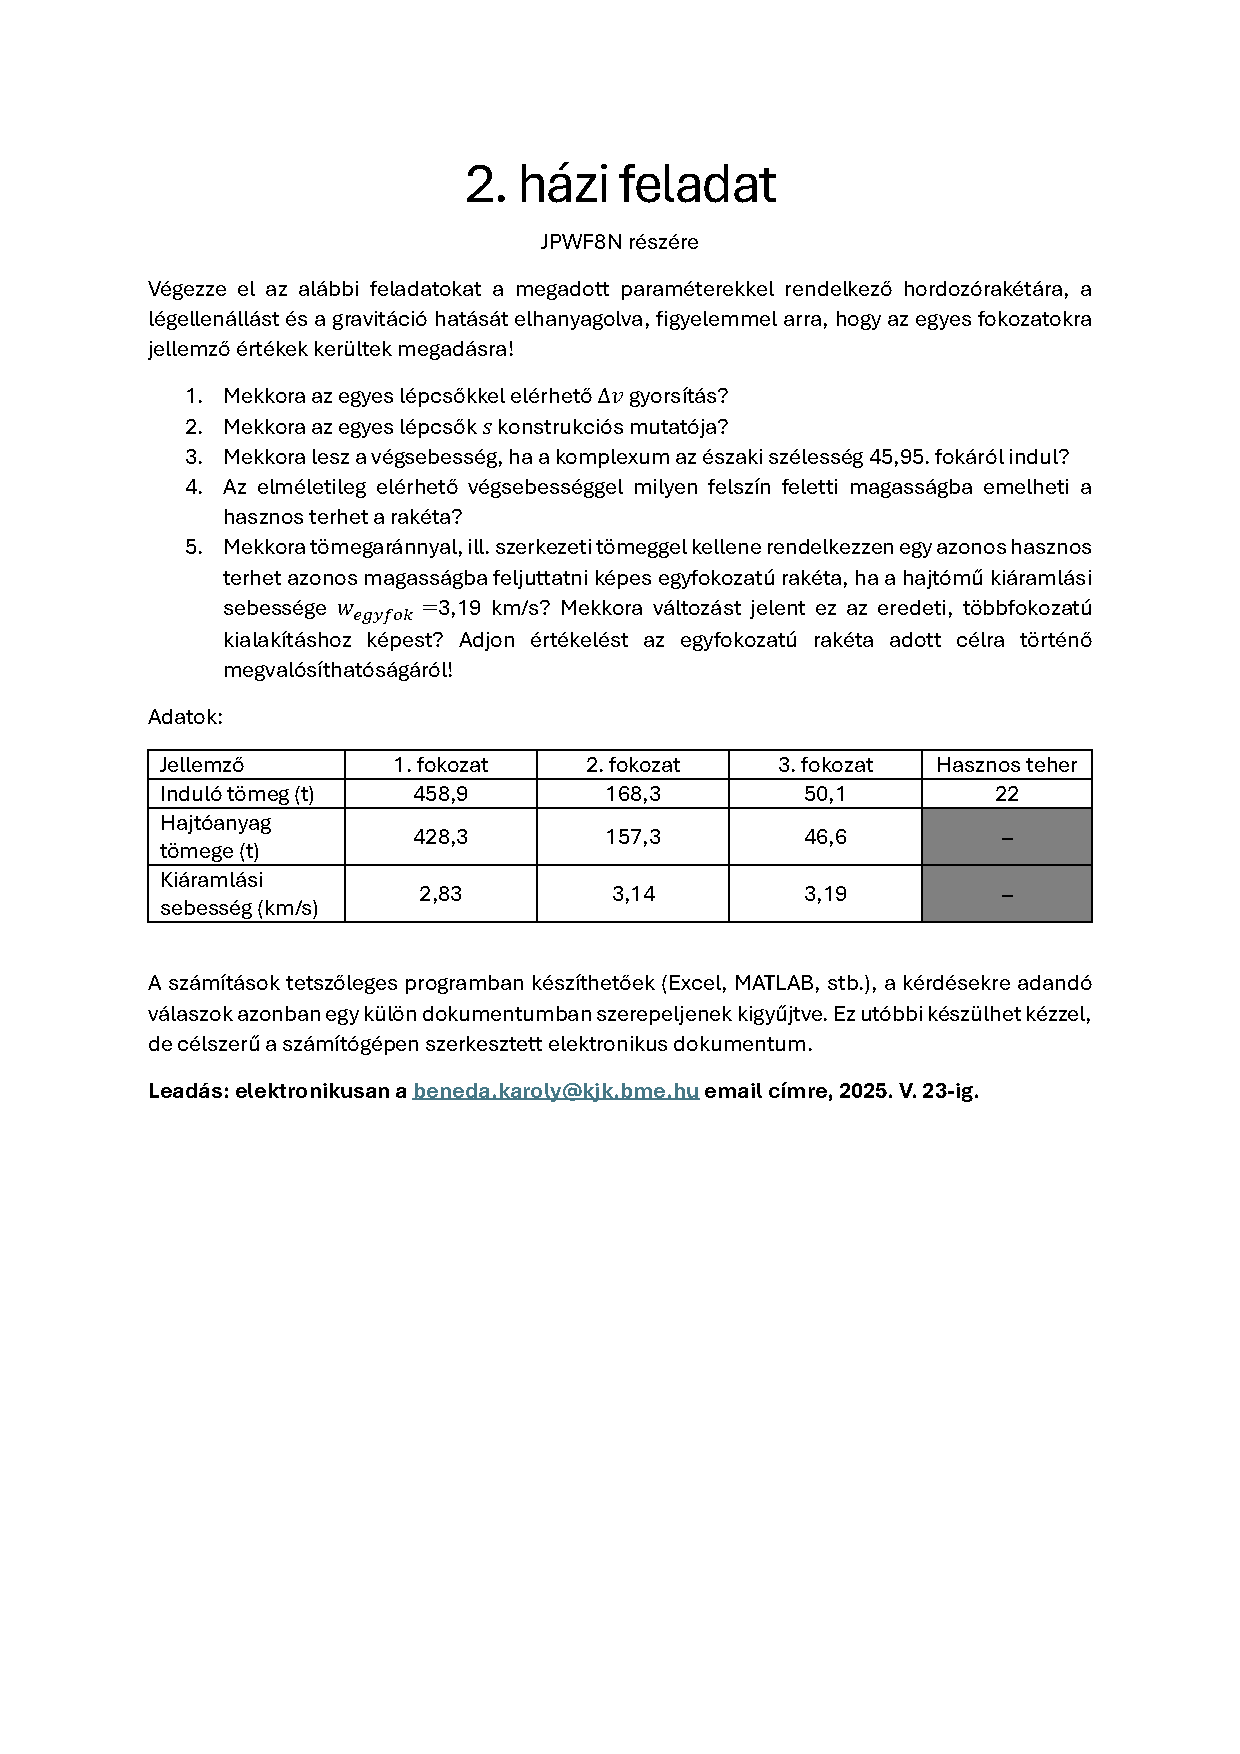
\includepdf[pages=-]{../handout/hw-2-JPWF8N.pdf}

% Section 1: Introduction
\section{Bevezetés}
A következő dokumentum a 2. házifeladat javítása a során elért eredményeket tartalmazza. Az egyszerű javítás érdekében itt már nem Jupyter notebook-ban, hanem Microsoft Excel táblázatban
végeztem el a számításokat.

Az táblázat a dokumentációval együt megtalálható a következő GitHub repository-ban:
\href{https://github.com/LaszloAbrok/rockets-and-rocket-engines}{rockets-and-rocket-engines repository}

\section{$\Delta$v számítása}

A sebességváltozás kiszámításához Ciolkovszkij egyenletét használtam:

\[
\Delta v_i = w_{e,i} \cdot \ln\left( \frac{m_{0,i}}{m_{f,i}} \right)
\]

\begin{itemize}
    \item \( w_{e,i} \) – az \(i\)-edik fokozat kiáramlási sebessége [m/s],
    \item \( m_{0,i} \) – az \(i\)-edik fokozat induló tömege [kg],
    \item \( m_{f,i} \) – az \(i\)-edik fokozat végső tömege [kg] (felsőbb fokozatok + hasznos teher + saját szerkezet).
  \end{itemize}

Ezáltal a következő értékek adódtak:
\begin{itemize}
    \item Első fokozat: \(\Delta v_1 = 2682.729669 \text{ m/s}\)
    \item Második fokozat: \(\Delta v_2 = 3470.610945 \text{ m/s}\)
    \item Harmadik fokozat: \(\Delta v_3 = 3315.608139 \text{ m/s}\)
\end{itemize}

\section{Konstrukciós mutató}

\[
s_i = \frac{m_{\text{szerk},i} + m_{\text{üza},i}}{m_{\text{szerk},i}}
\]

ahol:
\begin{itemize}
  \item \( m_{\text{szerk},i} \) – az \(i\)-edik fokozat szerkezeti tömege,
  \item \( m_{\text{üza},i} \) – az \(i\)-edik fokozat üzemanyag.
\end{itemize}

Ebből a következő értékek adódtak:
\begin{itemize}
    \item Első fokozat: \(s_1 = 14.99673203\)
    \item Második fokozat: \(s_2 = 15.3\)
    \item Harmadik fokozat: \(s_3 = 14.31428571\)
\end{itemize}

\section{Végsebesség}
\[
v_{\text{final}} = \sum_i \Delta v_i + v_{\text{E}} \cdot \cos(\varphi)
\]

Ahol:
\begin{itemize}
  \item \( \varphi \) – a szélesség (jelen esetben: \(45{,}95^\circ\)),
  \item \( v_{\text{E}} \) – Föld forgási sebessége az egyenlítőnél (kb. 465.11 m/s).
\end{itemize}

Ebből:
\[
v_{\text{final}} = 9792.333154 \text{ m/s}
\]


\section{Felszín feletti magasság}

A felszín feletti magasság kiszámításához előszőr a pályára állás sebességparaméterét számoltam ki.

\[
  k_i = \frac{v_i^2}{v_{ci}^2} = \frac{v_i^2}{\mu / r_i}
\]
  
ahol:
\begin{itemize}
    \item $k_i$ a sebességparaméter,
    \item $v_i$ a test pillanatnyi sebessége,
    \item $v_{ci}$ az adott $r_i$ sugarú körpályához tartozó körsebesség,
    \item $\mu$ a gravitációs paraméter ($\mu = G M$, ahol $M$ a Föld tömege),
    \item $r_i$ a pályamagasság.
\end{itemize}

Az pályamagasságot a Föld sugara és a felszín feletti magasság összege adja meg. Feltételezve, hogy 0 méterről indítjuk a rakétát a Föld sugarával számoltam.

A körsebesség a következő képpen adódott:
\[
  v_{ci} = \sqrt{\frac{\mu}{r_i}} = \sqrt{\frac{3.986 \cdot 10^{14} \text{ m}^3/\text{s}^2}{6.37 \cdot 10^6}} = 7.91 \cdot 10^3 \text{ m/s}
\]

A pályára állás sebességparamétere:

\[
  k_i = \frac{v_{\text{final}}^2}{v_{ci}^2} = \frac{(9792.333154 \text{ m/s})^2}{(7.91 \cdot 10^3 \text{ m/s})^2} = 1.53
\]

Ezt követően kiszámítottam a félnagytengely távolságát:

\[
  a = \frac{r_i}{2 - k_i} = \frac{6.37 \cdot 10^6 \text{ m}}{2 - 1.53 } = 1.36 \cdot 10^7 \text{ m}
\]

Ezután kiszámoltam az excentricitást:

\[
  e = \sqrt{k_i \cdot (k_i - 2) \cdot cos^2\gamma + 1} = 5.32 \cdot 10^{-2}
\]

Az félnagytengelyből meghatározható az apogeum sugara:

\[
  r_a = a \cdot (1 + e) = 1.36 \cdot 10^7 \text{ m} \cdot (1 + 5.32 \cdot 10^{-2}) = 2.09 \cdot 10^7 \text{ m}
\]

Az apogeum magasságát pedig a következő képpen kaphatjuk meg:

\[
  h_a = r_a - r_i = 2.09 \cdot 10^7 \text{ m} - 6.37 \cdot 10^6 \text{ m} = 1.45 \cdot 10^7 \text{ m} = 14500 \text{ km}
\]


\section{Egyfokozatú rakéta}

A tömegarányt a következő képlettel számoltam ki:
\[
z = \exp\left(\frac{\Delta v}{w_e}\right)
\]

Ahol:

\[
v_final = 9792.333154 \text{ m/s}
\]

és
\[
w_{egyfok} = 3.19 \text{ km/s} = 3190 \text{ m/s}
\]

\[
z_{egyfok} = 21.5353746
\]

Eközben a 3 fokozatú rakéta tömegaránya:

\[
  z_{3fok} = z_{13fok} \cdot z_{23fok} \cdot z_{33fok} = 2.580442804 \cdot 3.020100503 \cdot 2.82745098 = 22.0348814
\]

A tömegarány az egy és háromfokozatú rakéta esetében hasonló értékű.

Az induló tömeget pedig payload és z tömegarány segítségével számoltam ki:

\[
m_0 = z \cdot m_{\text{payload}} = 21.5353746 \cdot 22 \text{ t} = 473.7782412 \text{ t}
\]

Előszőr kiszámoltam a három fokozatú rakéta szerkezeti tömegének és üzemanyag tömegének arányát a következő módon:

\[
r = \frac{m_{\text{szerkezeti,3fok}}}{m_{\text{üza,3fok}}} = \frac{45.1 \text{ t}}{632.2 \text{ t}} = 0.071338184
\]

Ezután az egyfokozatú rakéta hajtóanyag tömegét számítottam ki:

\[
m_{\text{üza}} = \frac{m_0 - m_{\text{payload}}}{1 + r} = \frac{473.7782412 - 22}{1 + 0.071338184} = 421.6952667 \text{ t}
\]


A szerkezeti tömeget az induló tömeg, a hasznos teher és a üzemanyag kölönbségeként számítottam:

\[
m_{\text{szerkezeti}} = m_0 - m_{\text{payload}} - m_{\text{üza}} = 473.7782412 - 22 - 421.6952667 = 30.08297458 \text{ t}
\]

Az egyfokozatú és háromfokozatú rakéta tömegének aránya:

\[
\text{ratio} = \frac{m_{\text{szerk,3fok}}}{m_{\text{szerk,egyfok}}} =  \frac{30.08297458 \text{ t}}{45.1\text{ t}} = 0.667028261
\] 

Az egyfokozatú rakéta a számításaim alapján 30.08297458 tonna , amely a 45.1 tonnás háromfokozatú rakéta szerkezeti tömegének nagyjából 67\%-át teszi ki.
Ebben az esetben egy fokozatra hárul az egész payload pályára állítása. A szerkezettel ebben az esetben jóval nagobb terhelésbeli követelmények lépnek fel.
Ugyan a több fokozat esetén nagyobb lehet a meghibásodás esélye, mégis a három fokozat esetén van mód a fokozatok optimalizálására. Ugyan az egyfokozatú rendszer megvalósítható, célszerűbb lehet a többfokozatú rakéta használata.  

\end{document}